\documentclass[a4paper, 12pt, one column, aas_macros]{article}

%% Language and font encodings. This says how to do hyphenation on end of lines.
\usepackage[english]{babel}
\usepackage[utf8x]{inputenc}
\usepackage[T1]{fontenc}
\usepackage{aas_macros}

%% Sets page size and margins. You can edit this to your liking
\usepackage[top=1.3cm, bottom=2.0cm, outer=2.5cm, inner=2.5cm, heightrounded,
marginparwidth=1.5cm, marginparsep=0.4cm, margin=2.5cm]{geometry}

%% Useful packages
\usepackage{graphicx} %allows you to use jpg or png images. PDF is still recommended
\usepackage[colorlinks=False]{hyperref} % add links inside PDF files
\usepackage{amsmath}  % Math fonts
\usepackage{amsfonts} %
\usepackage{amssymb}  %
\usepackage{array} % enable column sizing
\usepackage[section]{placeins} %prevents figure jumping to end of document
\usepackage{float}
\usepackage[normalem]{ulem}

%% Citation package
\usepackage[authoryear]{natbib}
\bibliographystyle{abbrvnat}
\setcitestyle{authoryear,open={(},close={)}}


\title{NavUP System}
\author{
Bayanda Chakuma u11283212\\
Keegan Ferrett u15132847\\
Thomas Honiball u15348751\\
Keamogetswe Matsobe u16087004\\
Marin Peroski u13242475\\
Lucian Sargeant u15225560\\
John van Schalkwyk u14307317}

\begin{document}
\maketitle

\begin{abstract}
\begin{center}
Submitted in partial fulfillment of the requirements of COS301 \\Software Engineering
\end{center}
\end{abstract}

\section{Introduction}
Navigating through the University of Pretoria can be quite daunting for those who have never visited the institution before and for the first years alike. Lectures are spread across various buildings that contain a multitude of lecture halls. It definitely takes some time for a first year to become accustomed to the large ground space and especially when one’s timetable is packed back to back with lectures. Technology can be used yet again to simplify life and lessen the tediousness of learning where locations are on campus. NavUP is a mobile application that will help with just that.

\subsection{Purpose}
The purpose of this document is to provide a high level requirements specification of the NavUP navigational system. It will explain the basic purposes and features of the system as well as detailing the user interactions via modeling diagrams. This document is intended for stakeholders and developers of the system.

\subsection{Scope of the Project}
The system will be a mobile application for use by all students and visitors of the university. The system will be designed to provide faster navigational routes around the University of Pretoria Campus grounds by selecting shortest routes and accounting for pedestrian traffic density. By providing an intuitive interface and tools to automate the tasks of predictive route plotting the system will satisfy the users navigational needs while remaining user friendly.//Specifically this system is designed to allow users to select a location to navigate to. The software will facilitate  navigation by analysing crowd gathered locations from other application users along with wifi access points and signal strength to pinpoint the users location on campus grounds. This data is then used to calculate pedestrian traffic around campus and calculate the fastest route to the destination. The system also provides predictive location suggestions by gathering usage data if the user allows it too.

\subsection{Glossary}
\begin{center}
\begin{tabular}{|m{4cm}|m{10cm}|}
	\hline
    	\textbf{Term} & \textbf{Definition}\\\hline
        Crowdsourcing & The use of signals from multiple application users in order to gather datasets efficiently.\\\hline
        Heat Map & A representation of the density of people in a specified area.\\\hline
        
        Mobile Application & A software system developed to run specifically on mobile devices with sufficient software capability.\\\hline
        
		NavUP & A navigational system proposed within this System Requirements Specification document. An abbreviation of Navigation University of Pretoria.\\\hline
        
        Offline & A state indicating a device lacks connection to the internet.\\\hline
        Online & A state indicating a device has connection to the internet.\\\hline
        
        Profiling & Collecting data related to a person in order to form predictive formulae based on their behavioural patterns and routines\\\hline
        
        Pedestrian & An individual that travels without the aid of a vehicle along pathways\\\hline
        
        Reward & Incentive provided upon reaching a set goal\\\hline
        
        Software Requirements Specification & A document describing the requirements and constraints of a system. For example, this document.\\\hline
        
        Stakeholder & Any person with an interest in the project that is not a developer.\\\hline
        User & Any individual using the mobile application in accordance with its purpose.\\
  	\hline
\end{tabular}

\end{center}

\subsection{References}
IEEE. \textit{IEEE Std 830-1998 IEEE Recommended Practice for Software Requirements Specifications.} IEEE Computer Society, 1998.

\subsection{Overview}
The next chapter of this document will give an overview of the products functionality. It details informal requirements for the system and  establishes a context for the technical requirements specification.

The third chapter of this document is the Requirements Specification. It is written primarily for the developers and it will describe the various details of the product in technical terms.

These sections are intended for different audiences, but both refer to the same mobile application.

\section{Overall Description}

\subsection{Product Perspective}
The system consists of the End Users which can be students, lecturers and visitors of the University of Pretoria, all of which function as the same actor in the system, faculties and organizations on campus, which submit activities to the system. Thus the system consists of a total of 2 types of actors.
\newpage
\subsection{Product Functions}
\subsubsection{UC1 - Open Application Use Case}
\textbf{Diagram:}
\begin{figure}[H]
\centering
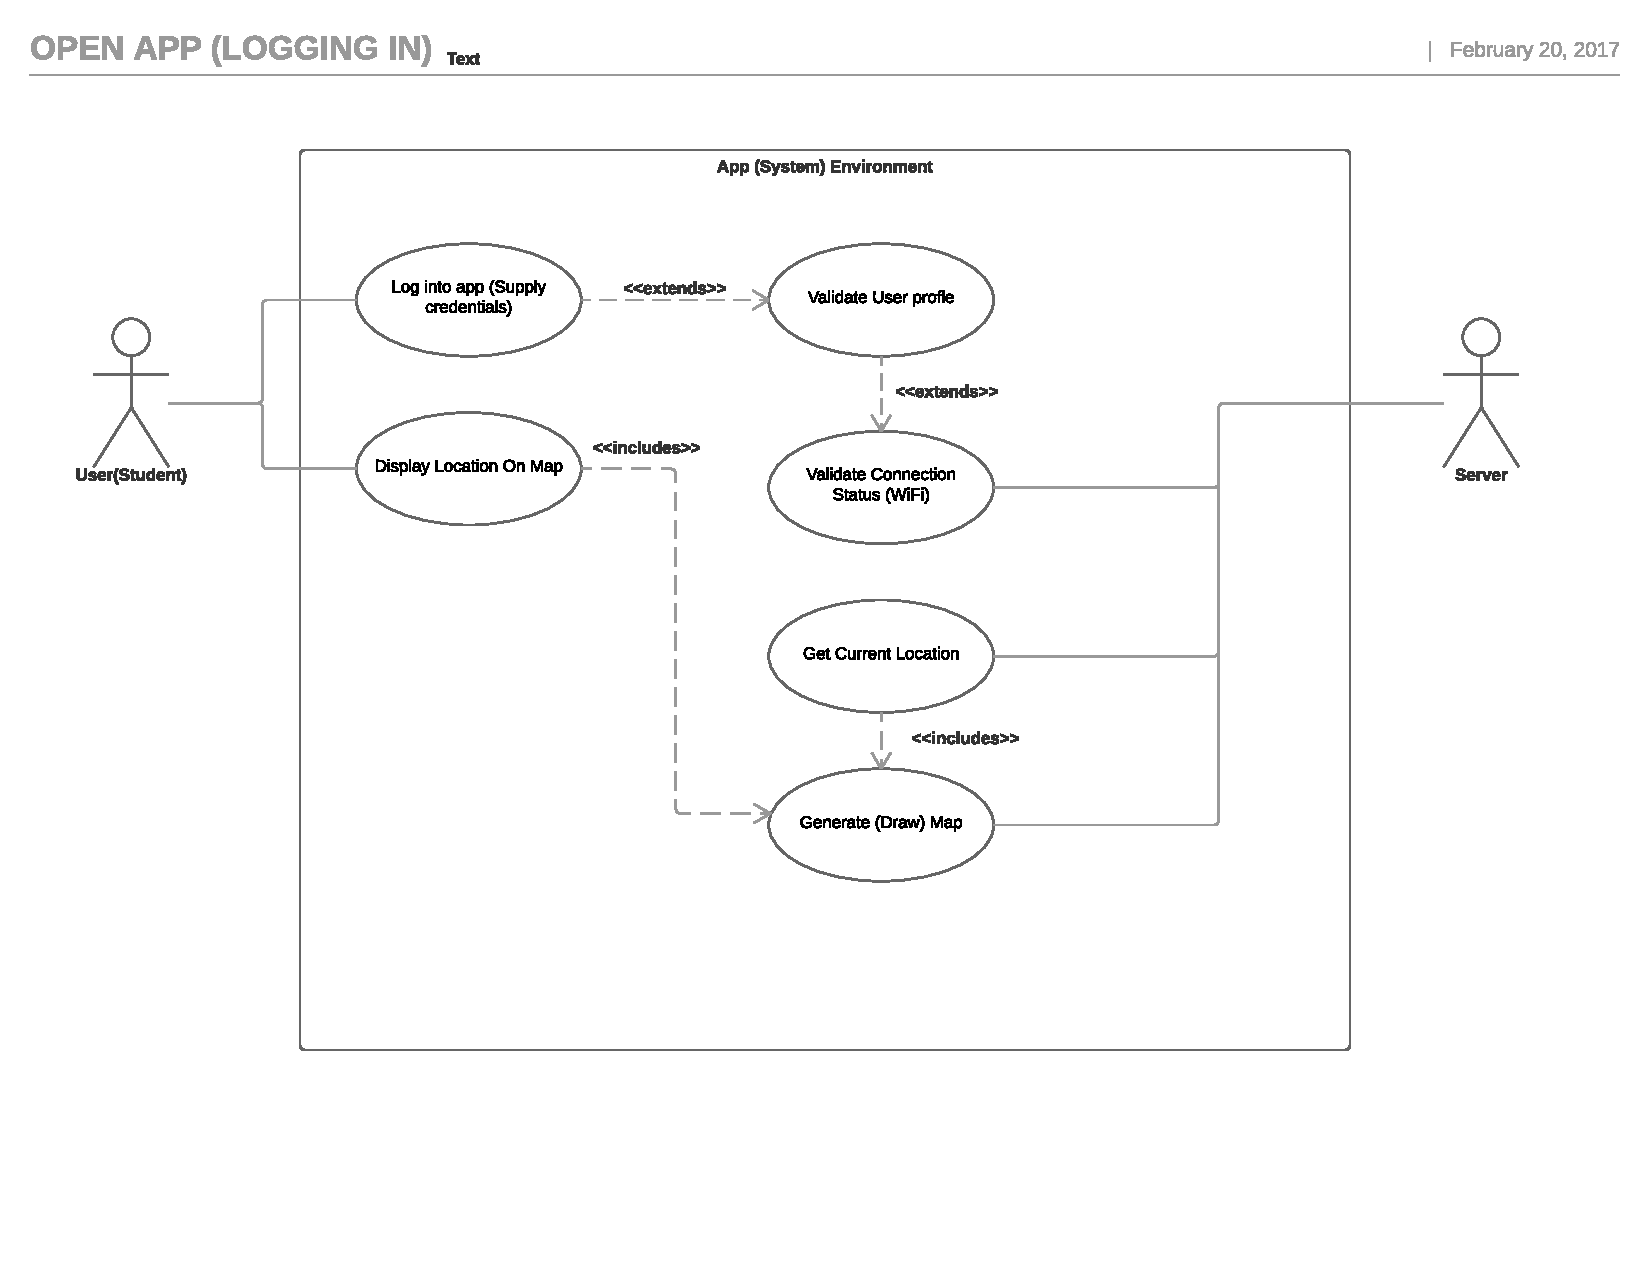
\includegraphics[width=0.8\textwidth]{App_Log_In_Use-Case.pdf}
\caption{UC1 - Open Application Use Case Model}
\end{figure}

\textbf{Brief Description}\\
User opens the app and is presented with a map of campus honed in on their current location as well as a search bar at the top to indicate where they would like to go.\\
\\\textbf{Initial Step-By-Step Description}
\begin{enumerate}
\item Map of the university is drawn. Location of user is gotten using GPS and/or WiFi and displayed on the map.
\end{enumerate}



\clearpage

\subsubsection{UC2 - Location Search Use Case}
\textbf{Diagram:}
\begin{figure}[H]
\centering
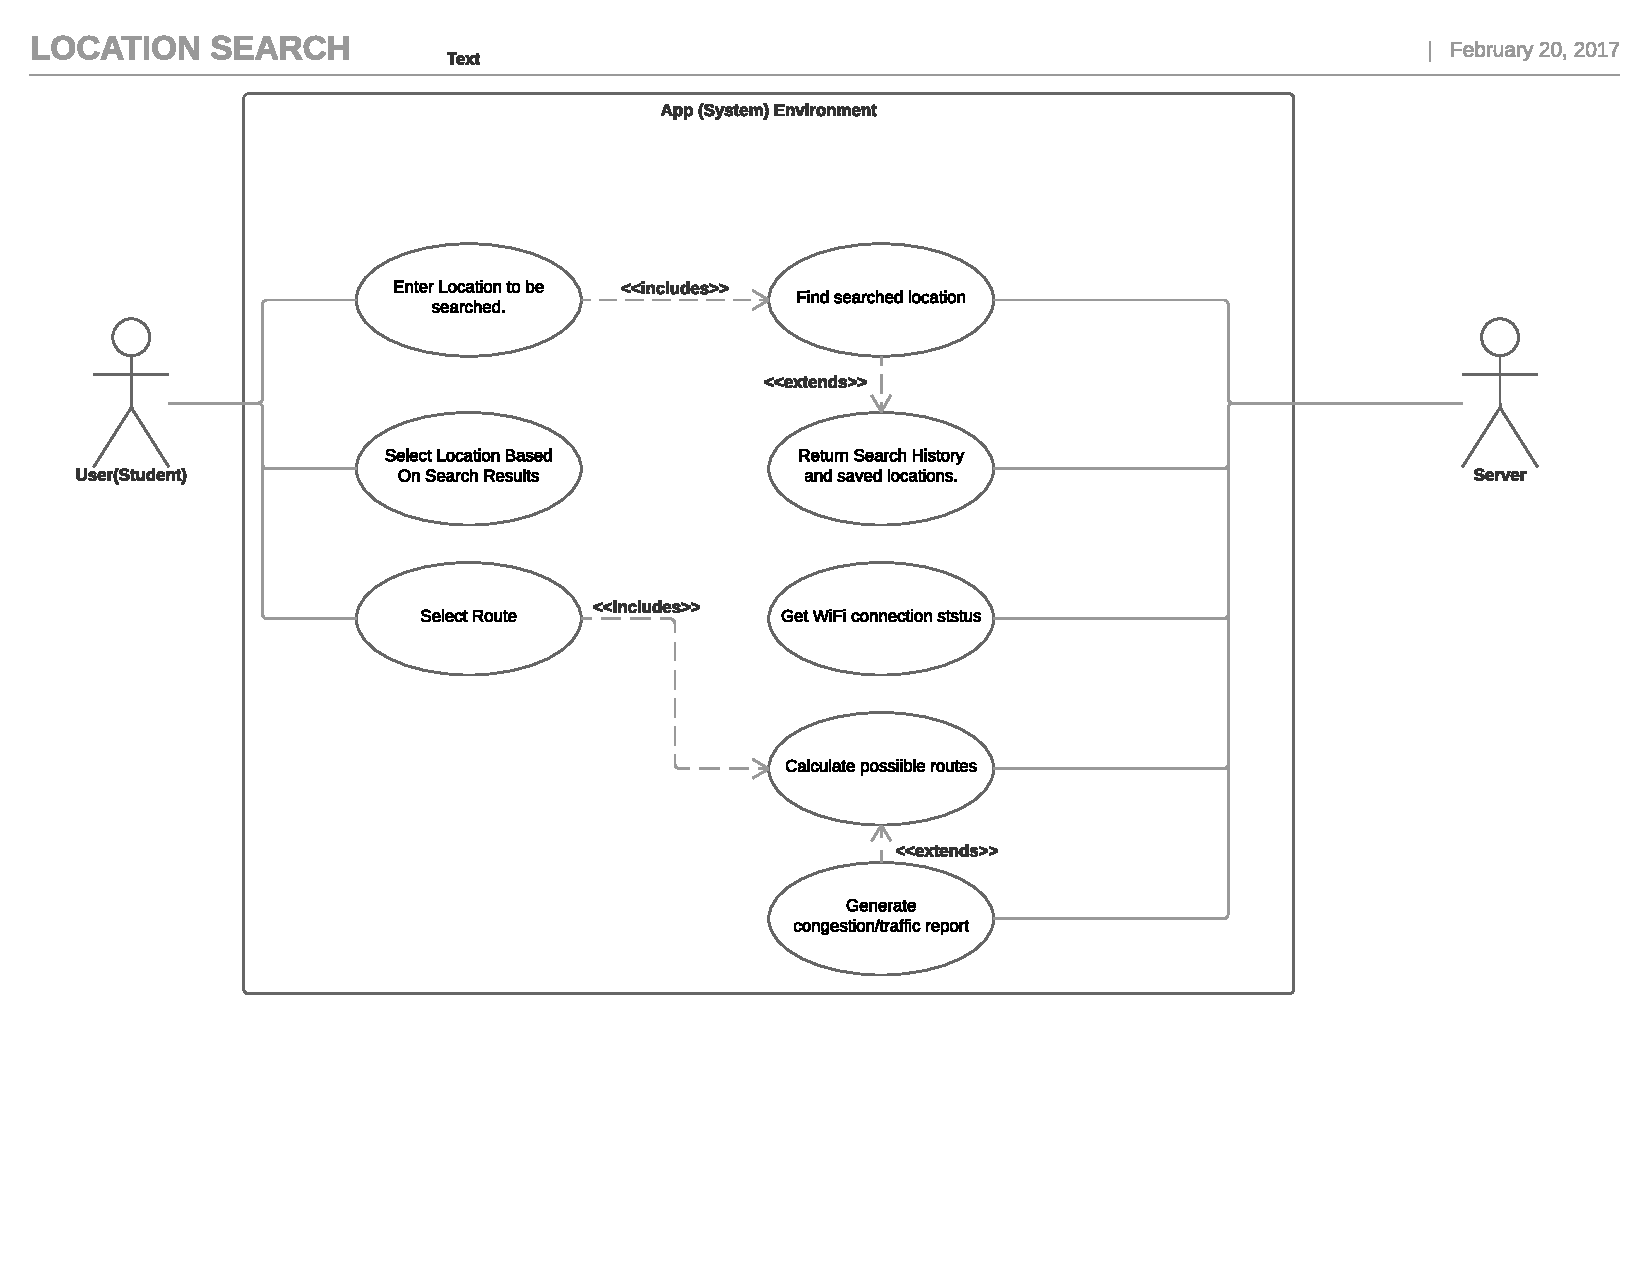
\includegraphics[width=0.8\textwidth]{Location_Search_Use-Case.pdf}
\caption{UC2-Location Search Use Case Model}
\end{figure}

\textbf{Brief Description}\\
User either types in the name of the location or selects it on the map by placing a “pin”. The user is then presented with routes to the destination if the destination exists.\\
\\\textbf{Initial Step-By-Step Description}\\
\begin{enumerate}
\item System displays drop down list of recently visited locations and suggested locations, as well as a search bar.
\item User either selects a choice from the drop down list or searches for another location.
\item System searches for location in database. If location is not found, report back to user and end user case, else, display location on university map and provide user with further options.
\end{enumerate}


\clearpage
\subsubsection{ UC3 - User Input Use Case}
\textbf{Brief Description}\\
The user can add information that describes what he or she is interested in with regards to activities or pastime events so that points of interest can be highlighted to them as they walk through campus. \\
\\\textbf{Initial Step-By-Step Description}\\
\begin{enumerate}
\item System displays form with options of what the user may be interested in.
\item User selects options from the form and then submits the results.
\item System analyzes the given information and come up with points of interest to display to the user when the user is deciding on a destination.
\end{enumerate}


\subsubsection{UC4 - User Timetable Use Case}
\textbf{Diagram:}
\begin{figure}[H]
\centering
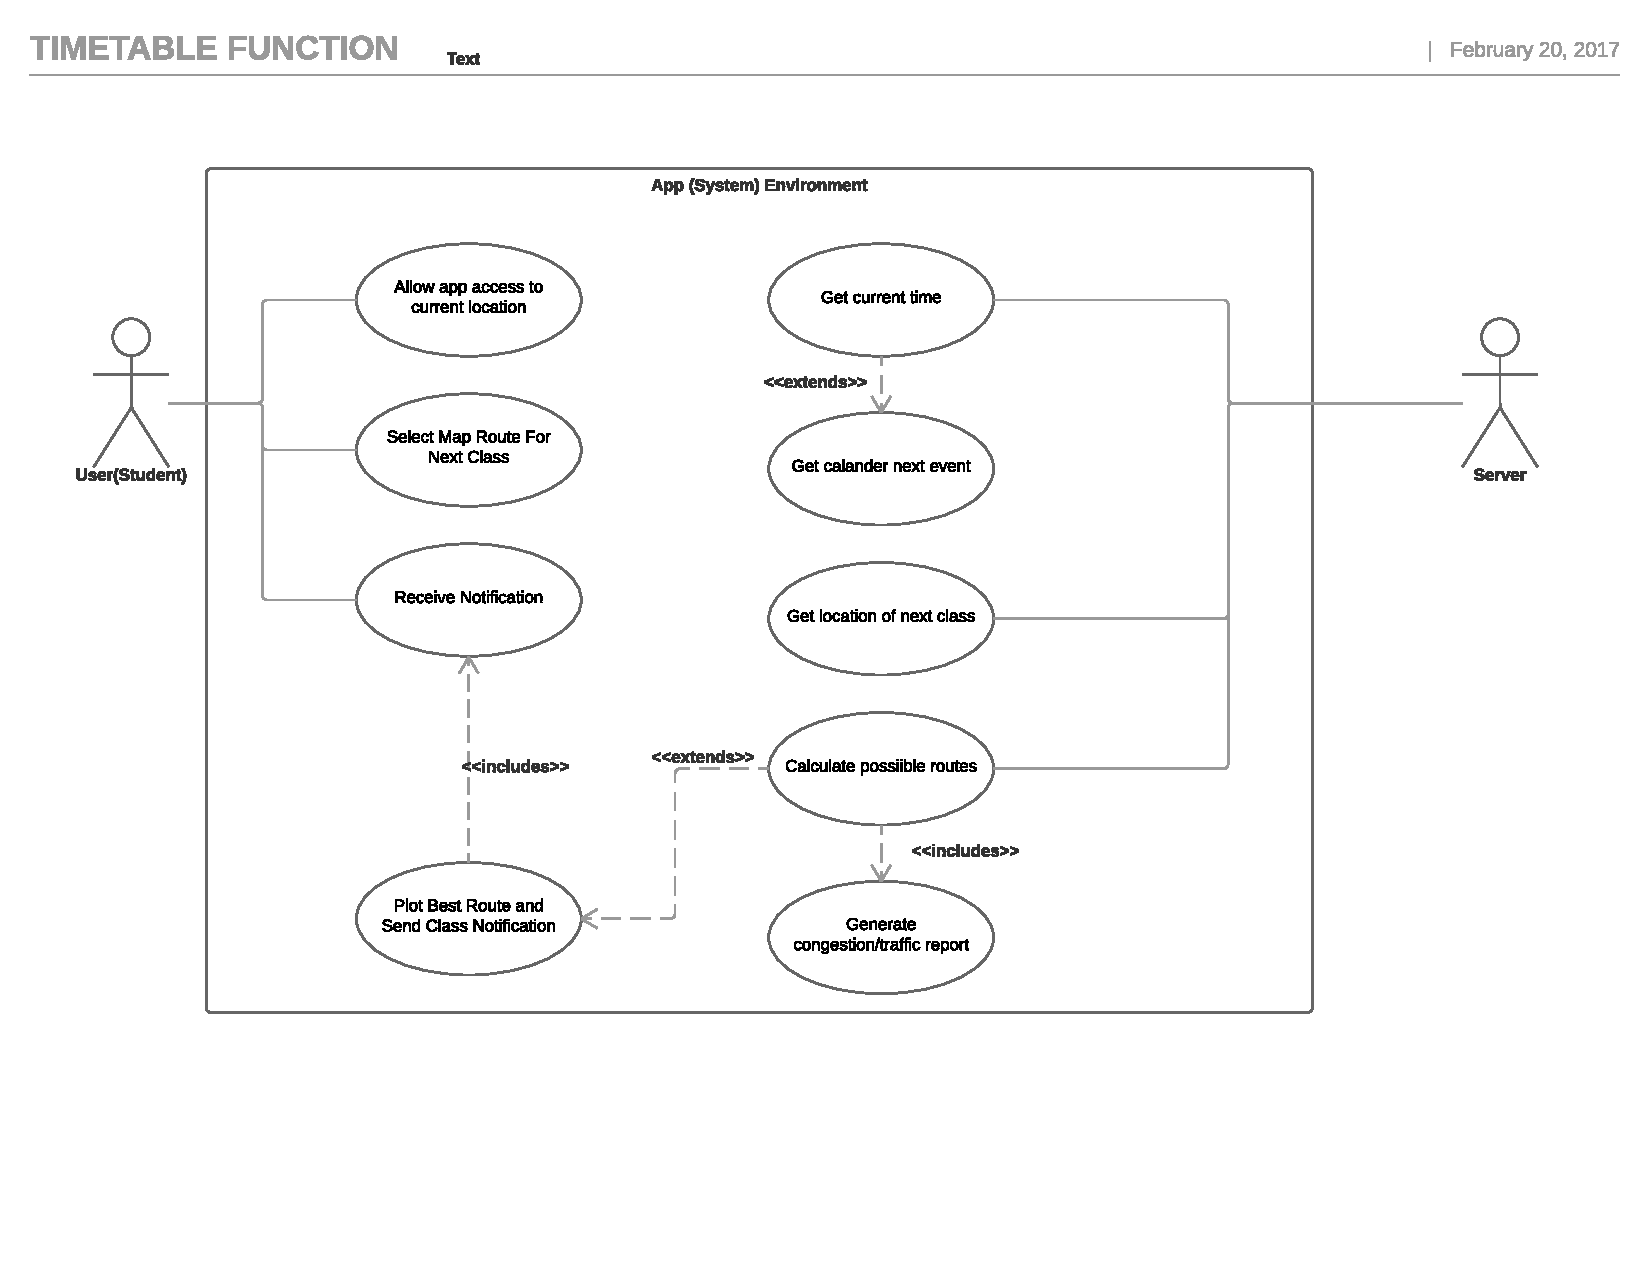
\includegraphics[width=0.8\textwidth]{Time_Table_Use-Case.pdf}
\caption{UC4 - User Timetable Use Case Model}
\end{figure}

\textbf{Brief Description}\\
The timetable can also be added by the user so that the route can automatically be determined based on his or her schedule.\\
\\\textbf{Initial Step-By-Step Description}\\
\begin{enumerate}
\item User selects option to add timetable
\item System displays a form to allow the user to submit a new class to their timetable.
\item User enters information about the class, such as module code, location, and time and then submits the information.
\item System adds class to user database and then refreshes the form for a new class.
\item User and system repeat steps 2 and 3 until all classes have been entered.
\item System can now provide a shortcut option when the user in searching for the location of their classes.
\end{enumerate}


\subsubsection{UC5 - Optimal Route and Traveling Use Case}
\textbf{Brief Description}\\
The user has requested a route to a destination and is presented with multiple options based on campus congestion. These route options will provide estimated time of arrival for each one allowing the user to make an informed decision.The optimal route will be shown and map changed based on whether the user is indoors or outdoors.\\
\\\textbf{Initial Step-By-Step Description}\\
Before this Use Case can be initiated the User must have requested a destination as per UC2
\begin{enumerate}
\item System displays multiple routes on the university map along with additional information about the route.
\item User selects a given route to the destination.
\item System displays chosen route, instructions and estimated time to reach selected  destination.
\item User begins along route.
\item System refreshes user location and reflect the location on the university map. Update estimated time based on user speed.
\item System relays next instruction.
\item User follows an instruction given by the application.
\item Repeat steps 5-7 until UC-8 occurs or navigation is aborted.
\end{enumerate}


\subsubsection{UC6 - Activities Use Case}
\textbf{Brief Description}\\
User selects a route and the estimated number of steps is added to their user profile in a game like fashion leading to possible rewards awarded by third party members.\\
\\\textbf{Initial Step-By-Step Description}\\
User must have initiated and completed UC2 or have initiated UC5 up to step 3
\begin{enumerate}
\item System adds estimated number of steps to the user profile. If user is eligible, system presents a reward to the user.
\item If reward is presented, the user can collect/store the reward.
\item System records the state of the user’s reward (stored/ used).
\end{enumerate}

\subsubsection{UC7 - User Based Augmented Reality Use Case}
\textbf{Brief Description}\\
As the user travels along their route and passes certain landmarks they will be presented with certain information about these landmarks. For example if they pass the music department they will be given the option to see upcoming performances. This will be based on the interests that they have specified on their profiles.\\
\\\textbf{Initial Step-By-Step Description}\\
Before this Use Case can be initiated the user must have accepted the terms and conditions related to data usage and must be near a landmark
\begin{enumerate}
\item Systems tracks user location as the are on route to their destination. If user gets near a possible point of interest, notify them and provide information about the landmark.
\item User acknowledges the notification. If events are available at the landmark the user can select any to be added to a calendar.
\item If any event was selected system adds it to the users calendar.
\end{enumerate}

\subsubsection{UC8 - End Point Use Case}
\textbf{Brief Description}\\
Once the user reaches their destination navigation will stop until the user enters in a new location or the location is pulled from their timetable information.\\
\\\textbf{Initial Step-By-Step Description}\\
This Use Case cannot be initiated unless UC5 has completed immediately prior
\begin{enumerate}
\item System realises user has reached the destination when users location is close enough to the location of the entered destination. Displays information about the trip, such as duration, distance travelled, average speed, etc.
\item User acknowledges that they have arrived at the destination.
\item System UI resets and awaits a new destination from the user.
\end{enumerate}


\section{Specific Requirements}


\subsection{Functionality}

\subsubsection{Functional}
\begin{enumerate}
\item R1 - Basic User Profiling without violating user’s personal information

\begin{itemize}
\item The system shall allow users to create a profile and set credentials
\item The system shall authenticate user credentials to view profile
\item The system shall allow the user to update profile
\item The system shall display frequently searched destinations by the user in the profile
\item The system shall allow the user to register for push notifications
\end{itemize}

\item R2 - Indoor Functionality
\begin{itemize}
\item The system shall provide a map of the current floor the user is on.
\item The system shall provide the user's location within the floor.
\item The system shall allow the user to specify a classroom on the floor.
\end{itemize}

\item R3 - Outdoor Functionality
\begin{itemize}
\item The System shall provide the location of the user on campus
\item The system shall provide building identification
\end{itemize}

\item R4 -Heat Map Signatures of Crowds

\begin{itemize}
\item The system shall allow the user to view possible traffic and crowed congested areas
\end{itemize}
 

\item R5 -Detailed map of the university (both indoor maps and outdoor maps)

\begin{itemize}
\item The system shall allow the user to view a detailed map of the University
\end{itemize}

\item R7 -Ability to direct user to specific class rooms and buildings

\begin{itemize}
\item The system shall enable the user to enter search text (destination) on the screen
\item The system shall allow the user to select preferred route to destination
\item The system shall notify the user when there is no matching search result
\end{itemize}

\item R8 -Should use quickest path (least congested)

\begin{itemize}
\item The system shall calculate the optimum path to get to the destination
\end{itemize}

\item R9 -Provide information on any local landmarks or events

\begin{itemize}
\item The system shall notify the user of any activities happening on campus
\end{itemize}

\item R10 -Use WiFi as well as GPS to determine location

\begin{itemize}
\item Full functionality and performance is determined by the use of Wi-Fi and GPS 
\item Response time for loading the NavUP will be determined by the internet strength
\end{itemize}

\item R11 -Be able to determine height location in buildings

\begin{itemize}
\item The system shall enable the user to view their current floor-level height in buildings
\end{itemize}

\item R14 - Provide a tour around campus
\begin{itemize}
\item The system shall provide a basic tour of the campus grounds, covering all the important buildings and landmarks.
\end{itemize}

\end{enumerate}

\subsection{Non-Functional}
\begin{enumerate}

\item R6 -Accurate directional navigation both indoors and outdoors
\begin{itemize}
\item The system will allow the user to set destination
\item The system shall allow the use of icons and tool bars
\item The system shall direct the user to the correct destination
\end{itemize}

\item R12 -When not connected to network have basic offline functionality 

\begin{itemize}
\item The system will enable the user to view profile
\item The system will allow the user to receive push notifications
\end{itemize}

\item R13 -Third party reward system for performing certain actions
\end{enumerate}


\subsection{Performance}

The NavUp App has to be downloaded from Playstore or iTunes to run on smartphone devices.The devices have to be connected to Tuks Wi-fi for the user to access and use the application.The Wi-Fi internet connection strength will determine the efficiency of the app.

\subsection{Design Constraints}

\subsubsection{Navigation Application Development}
The application is to be built using a webpage based on IDE (Intergrated Developmet Environment)

\subsubsection{Navigation Application}
\begin{enumerate}
\item The user is required to have basic computer skills to understand and use the App
\item The App must allow the user access it easily without violating users personal information 
\item Response time for functions of the App should not take long
\end{enumerate}

\subsection{Software System Attributes}
 \begin{itemize}
 
\item Reliability
\begin{itemize}
\item NavUP App should be reliable in terms of returning accurate results.
\end{itemize} 


\item Availability
\begin{itemize}
\item NavUP App shoud always be available when used, exceptions are when there is a network failure.
\item For the App to be available it should always be connected to Tuks Wi-Fi.
\item App should be connected to GPS to get the user's location, calculate the destination and determine shorted route.
\end{itemize} 

\item Security
\begin{itemize}
\item Users input information should not be easily identifiable if it the system is compromised.
\item The System should limit user details to essentials needed for the app to work. 
\end{itemize} 

\item Maintainability
\begin{itemize}
\item The code of the Application should be written in a way to acccomodate the future implementation functions.
\item Test Environment should be built to test different fuctions of the application.
\end{itemize} 

\item Portability 
\begin{itemize}
\item NavUp App should be portable with Android and iOS.
\end{itemize} 
\end{itemize} 

\subsection{Other Requirements}
\begin{enumerate}

\item R2 -Indoor functionality
\begin{enumerate}
\item Detect User's Location
\item Find  routes
\end{enumerate}

\item R3 -Outdoor functionality


\end{enumerate}




\newpage
\section{Requirements Traceability Matrix}
\useunder{\uline}{\ul}{}
\begin{table}[H]
	\centering
	\caption{Traceability Matrix}
	\begin{tabular}{l|l|l|l|l|l|l|l|l|}
		\cline{2-9}
		                                                 & \multicolumn{8}{c|}{{\ul \textbf{Use Cases}}} \\ \hline
		\multicolumn{1}{|l|}{{\ul \textbf{Requirement}}} & UC1 & UC2 & UC3 & UC4 & UC5 & UC6 & UC7 & UC8 \\ \hline
		\multicolumn{1}{|l|}{R1}                         &     &     & X   & X   &     & X   & X   &     \\ \hline
		\multicolumn{1}{|l|}{R2}                         & X   & X   &     & X   & X   &     & X   & X   \\ \hline
		\multicolumn{1}{|l|}{R3}                         & X   & X   &     & X   & X   &     & X   & X   \\ \hline
		\multicolumn{1}{|l|}{R4}                         &     &     &     &     & X   &     &     & X   \\ \hline
		\multicolumn{1}{|l|}{R5}                         & X   & X   &     & X   & X   &     &     & X   \\ \hline
		\multicolumn{1}{|l|}{R6}                         &     &     &     &     & X   &     &     & X   \\ \hline
		\multicolumn{1}{|l|}{R7}                         &     &     &     & X   & X   &     &     & X   \\ \hline
		\multicolumn{1}{|l|}{R8}                         &     &     &     &     & X   &     &     & X   \\ \hline
		\multicolumn{1}{|l|}{R9}                         &     &     & X   &     &     &     & X   &     \\ \hline
		\multicolumn{1}{|l|}{R10}                        & X   &     &     &     & X   &     & X   & X   \\ \hline
		\multicolumn{1}{|l|}{R11}                        & X   & X   &     &     & X   &     &     & X   \\ \hline
		\multicolumn{1}{|l|}{R12}                        &     & X   &     &     &     &     &     &     \\ \hline
		\multicolumn{1}{|l|}{R13}                        &     &     &     &     &     & X   &     &     \\ \hline
	\end{tabular}
\end{table}
\newpage
\section{User-System Modelling}
  UC1 - Open Application \hfill \break
  \begin{tabular}{ |p{5.5cm}|p{5.5cm}| }
    \hline
    \multicolumn{1}{|c|}{Actor} & \multicolumn{1}{c|}{System} \\ \hline
     & 0. Map of the university is drawn. Location of user is gotten using GPS and/or WiFi and displayed on the map. \\ \hline
  \end{tabular}
\hfill \break \hfill \break \hfill \break
  UC2 - Location Search \hfill \break
  \begin{tabular}{ |p{5.5cm}|p{5.5cm}| }
    \hline
    \multicolumn{1}{|c|}{Actor} & \multicolumn{1}{c|}{System} \\ \hline
     &0. Drop down list of recently visited locations and suggested locations, as well as a search bar.\\ \hline
     1. User either selects a choice from the drop down list or searches for another location. &2. Searches for location in database. If location is not found, report back to user and end user case, else, display location on university map and provide user with further options.\\ \hline
  \end{tabular}
\hfill \break \hfill \break \hfill \break
  UC3 - User Input \hfill \break
  \begin{tabular}{ |p{5.5cm}|p{5.5cm}| }
    \hline
    \multicolumn{1}{|c|}{Actor} & \multicolumn{1}{c|}{System} \\ \hline
     &0. Displays a form to allow the user to submit a new class to their timetable.\\ \hline
     1. Enters information about the class, such as module code, location, and time and then submits the information. &2. Adds class to user database and then refreshes the form for a new class.\\ \hline
     3. Repeats process until all classes have been entered. &4. Can now provide a shortcut option when the user in searching for the location of their classes.\\ \hline
  \end{tabular}

\newpage
  UC4 - User Timetable \hfill \break
  \begin{tabular}{ |p{5.5cm}|p{5.5cm}| }
    \hline
    \multicolumn{1}{|c|}{Actor} & \multicolumn{1}{c|}{System} \\ \hline
     &0. Displays a form to allow the user to submit a new class to their timetable.\\ \hline
     1. Enters information about the class, such as module code, location, and time and then submits the information. &2. Adds class to user database and then refreshes the form for a new class.\\ \hline
     3. Repeats process until all classes have been entered. &4. Can now provide a shortcut option when the user in searching for the location of their classes.\\ \hline
  \end{tabular}

\hfill \break \hfill \break \hfill \break
  UC5 - Optimal Route and Traveling \hfill \break
  \begin{tabular}{ |p{5.5cm}|p{5.5cm}| }
    \hline
    \multicolumn{1}{|c|}{Actor} & \multicolumn{1}{c|}{System} \\ \hline
     &0. System displays multiple routes on the university map along with additional information about the route.\\ \hline
     1. User selects a given route to the destination. &2. Displays chosen route, instructions and estimated time to reach selected destination.\\ \hline
     3. Begins along route.&4. Refresh user location and reflect the location on the university map. Update estimated time based on user speed.\\ \hline
     5. Follows an instruction given by the application.&6. Refresh user information and display next instruction.\\ \hline
  \end{tabular}
\hfill \break \hfill \break \hfill \break
  UC6 - Activities \hfill \break
  \begin{tabular}{ |p{5.5cm}|p{5.5cm}| }
    \hline
    \multicolumn{1}{|c|}{Actor} & \multicolumn{1}{c|}{System} \\ \hline
     &0. Estimated number of steps is added to the user profile. If user is eligible, system presents a reward to the user.\\ \hline
    1. If reward is presented, the user can collect/store the reward.&2. Record the state of the user’s reward (stored/ used).\\ \hline
  \end{tabular}
\hfill \break \hfill \break \hfill \break
\newpage
  UC7 - User Based Augmented Reality \hfill \break
  \begin{tabular}{ |p{5.5cm}|p{5.5cm}| }
    \hline
    \multicolumn{1}{|c|}{Actor} & \multicolumn{1}{c|}{System} \\ \hline
     &0. Tracks user location as the are on route to their destination. If user gets near a possible point of interest, notify them and provide information about the landmark.\\ \hline
     1. Acknowledges the notification. If events are available at the landmark the user can select any to be added to a calendar. &2. If any event was selected added it to the users calendar.\\ \hline
  \end{tabular}
\hfill \break \hfill \break \hfill \break
  UC8 - End Point \hfill \break
  \begin{tabular}{ |p{5.5cm}|p{5.5cm}| }
    \hline
    \multicolumn{1}{|c|}{Actor} & \multicolumn{1}{c|}{System} \\ \hline
     &0. Realises user has reached the destination when users location is close enough to the location of the entered destination. Displays information about the trip, such as duration, distance travelled, average speed, etc.\\ \hline
     1. User acknowledges that they have arrived at the destination.&2. UI resets and awaits a new destination from the user.\\ \hline
  \end{tabular}
\end{document}
